\newpage
\appendix
\subsection{State-based RL Expert Training Details}
\label{sec:state-rl}
\textbf{Model Architecture:} Since DrM~\cite{xudrm} is inherently designed as a visual reinforcement learning algorithm, we replace its visual encoder with a three-layer multilayer perceptron (MLP), employing ELU as activation functions. Meanwhile, the network architectures and hyperparameters of the Actor, Critic, and V-network remain unchanged.

\textbf{Training Hyperprameters:} We employ the identical set of reinforcement learning hyperparameters as those in the original visual RL implementation, without conducting any further hyperparameter tuning specifically for DrM in our experiments. For PPO, we employ the implementation available in MuJoCo Playground~\cite{mujoco_playground_2025}, which is built upon the RSL-RL framework~\cite{rudin2022learning}.


\textbf{Reward Hyperparameters:} The reward hyperparameters are listed in Table~\ref{table:reward_hype}. In addition to the proposed reward terms, contact information is incorporated during training on teleoped-motion tasks to tune the distance-chain reward coefficients.
\begin{table}[h]
    \centering
    \caption{Reward Hyperparameters}
    \begin{tabular}{c|c}
    \hline
    Description & Value \\
    \hline
        contact predefined threshold $N_{\text{num}}$ & $2$ \\
        object position reward coefficient $k_{1}$ & $1$ \\
        object orientation reward coefficient $k_{2}$ & $1$ \\
        coefficient of penalty & $1e-3$ \\

    \end{tabular}
    \label{table:reward_hype}
\end{table}

\textbf{Observations of RL training:} The dimensions of the observation for training expert state-based policy are provided in Table~\ref{table:obs_all}. 
\begin{table}[h]
    \centering
    \caption{Observation Descriptions}
    \begin{tabular}{c|c}
    \hline
    Description & Dimension \\
    \hline
        arm joint position  & $12$ \\
        hand joint position & $36$ \\
        arm joint velocity & $12$ \\
        hand joint velocity & $36$ \\
        hand position & $6$ \\
        hand quaternion & $8$ \\
        object-centric distance chain & $72$ \\
        contact information & $24$ \\
        actuator value & $24$ \\
        time & $1$ \\
        distance with the reference  & $10$ \\
        hand position in reference & $6$ \\
        hand quaternion in reference & $8$ \\
        object position in reference & $3$ \\
        object quaternion in reference & $4$ \\

    \end{tabular}
    \label{table:obs_all}
\end{table}

\textbf{Action space:} Actions are parameterized as a six-dimensional end-effector pose: the first three are translation, and the last three are Euler angles. For residual actions,  the translation range is $[-0.01, 0.01]$ m and the orientation range is $[-0.04, 0.04]$ rad. Regarding the actions in trajectories, teleoperated motions are scaled to $[-0.2, 0.2]$ m and $[-0.4, 0.4]$ rad, whereas motions derived from video and mocap are scaled to $[-1, 1]$ m and $[-1, 1]$ rad. 

\subsection{Human Motion Data Pre-processing}
We apply downsampling to the collected human motion data in order to reduce episode length and redundant steps, thereby facilitating more efficient policy learning of task skills. For human video data, particularly when involving symmetric objects, we observe that the FoundationPose~\cite{wen2024foundationpose} estimator may introduce rotational ambiguities during pose prediction. To address this, we preprocess the object pose trajectories to mitigate pose discrepancies induced by object symmetry.

\subsection{Task Description}
We design a suite of tasks specifically tailored for bimanual dexterous hand manipulation. Below, we provide a detailed description of each individual task:

\textit{Bottle Handover}: The robot is required to execute a hand-to-hand transfer, passing a bottle from the right hand to the left, followed by accurately placing it into a designated container.

\textit{Clean Table}: The task entails sequentially picking up both a bottle and a cup from the tabletop and placing them into a box.  

\textit{Scan Bottle}: The robot must first grasp a bottle from the table, subsequently pick up a scanning device, and then complete a bottle-scanning action. 

\textit{Place Drawer}: This task requires the robot to open a drawer, place multiple objects from the tabletop into the drawer sequentially, and finally close the drawer. 

\textit{Pour Teapot}: The robot is required to perform a pouring action by transferring liquid from a container into a teapot. 

\textit{Clean Plate}: The robot must grasp both a plate and a dishcloth, and then execute a wiping motion over the plate’s surface. 

\textit{Putoff Burner}: This task involves picking up a burner cap and performing a two-step extinguishing sequence to put out an alcohol burner

\textit{Flower Vase}: The robot is required to insert a flower into a vase. 




\subsection{DAgger Training Details}
\label{sec:dagger}
We list the hyperparameters of DAgger training in Table~\ref{table:dagger_hype}. Moreover, we randomize the camera viewpoint to account for discrepancies between the simulated and real-world camera poses. The action head is a three-layer MLPs with two hidden layers using ReLU activations; its outputs are subsequently squashed with a tangent activate function to enforce bounded actions in the target action space. 
\begin{table}[h]
    \centering
    \caption{DAgger Training Hyperparameters}
    \resizebox{0.4\textwidth}{!}{\begin{tabular}{c|c}
    \hline
    Description & Value \\
    \hline
        Buffer size  & $1e^{5}$ \\
        Learning rate  & $1e^{-4}$ \\
        Optimizer  & Adam \\
        Scheduler adjusted probability $p$ & $0.93$ \\
        Optimizer eps & $1e^{-8}$ \\
        Batch size & $256$ \\
        Action repeat & $1$ \\
        Frame stack & $3$ \\
        Depth threshold distance $\mathbf{d}$ & $0.9$ to $1.1$ \\

    \end{tabular}}
    \label{table:dagger_hype}
\end{table}

The DAgger training action objective is:
\begin{equation}
  \mathcal{L}_{\mathrm{act}}(\theta)
  = \mathbb{E}_{(\mathbf{o}_t,\mathbf{a}^{\star}_t)\sim\mathcal{D}}
    \Big[\,\|\mathbf{a}_t-\mathbf{a}^{\star}_t\|_2^{2}\,\Big]
  + \mathbb{E}_{(\mathbf{o}_t,\mathbf{a}^{\star}_t)\sim\mathcal{D}}
    \Big[\,\|\mathbf{a}_t-\mathbf{a}^{\star}_t\|_1\,\Big],
  \label{eq:act_loss_expect}
\end{equation}

where $\mathbf{a}_t=\pi_{\theta}(\mathbf{o}_t)$, and $\mathbf{a}^{\star}_t$ is the expert action.  

\subsection{Navigation Details}
\label{sec:nav}
We adopt the same navigation configuration as employed in ViNT. For localization, we first capture RGB-D images of the target position. Then, during navigation, the images recorded along the reference trajectories serve as goal observations for inferring the subsequent actions. In addition, we configure the number of waypoints to $4$ and set the radius to $5$, tailoring these parameters to the operational characteristics of our mobile platform.

\subsection{Instance Generalization}
\begin{figure}[t]
  \centering
  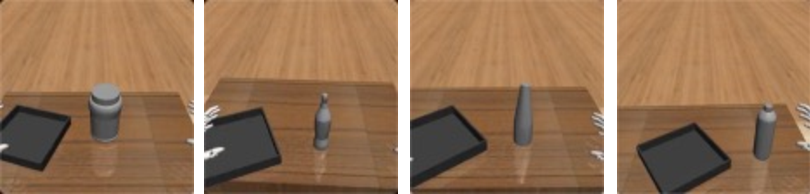
\includegraphics[width=1.0\linewidth]{figures/obj_generalization_pic.pdf}
  \caption{ \textbf{Object generalization visualization.} To help the policy adapt to different object shapes, we randomize each object’s geometry during training to prompt the policy to adjust its actions accordingly.}
  \label{fig:obj_generalization}
\end{figure}
We also conduct experiments to assess the object-level generalization capability of our approach. For the handover task, we select several bottles from the UniDexGrasp++ dataset~\cite{wan2023unidexgrasp++} and introduce randomized variations in bottle shapes during each environment reset. The corresponding visualizations are presented in Figure~\ref{fig:obj_generalization}. The trained policy, distilled via the DAgger framework, demonstrates zero-shot generalization to bottles of varying shapes in real-world settings.


\begin{figure*}[t]
  \centering
  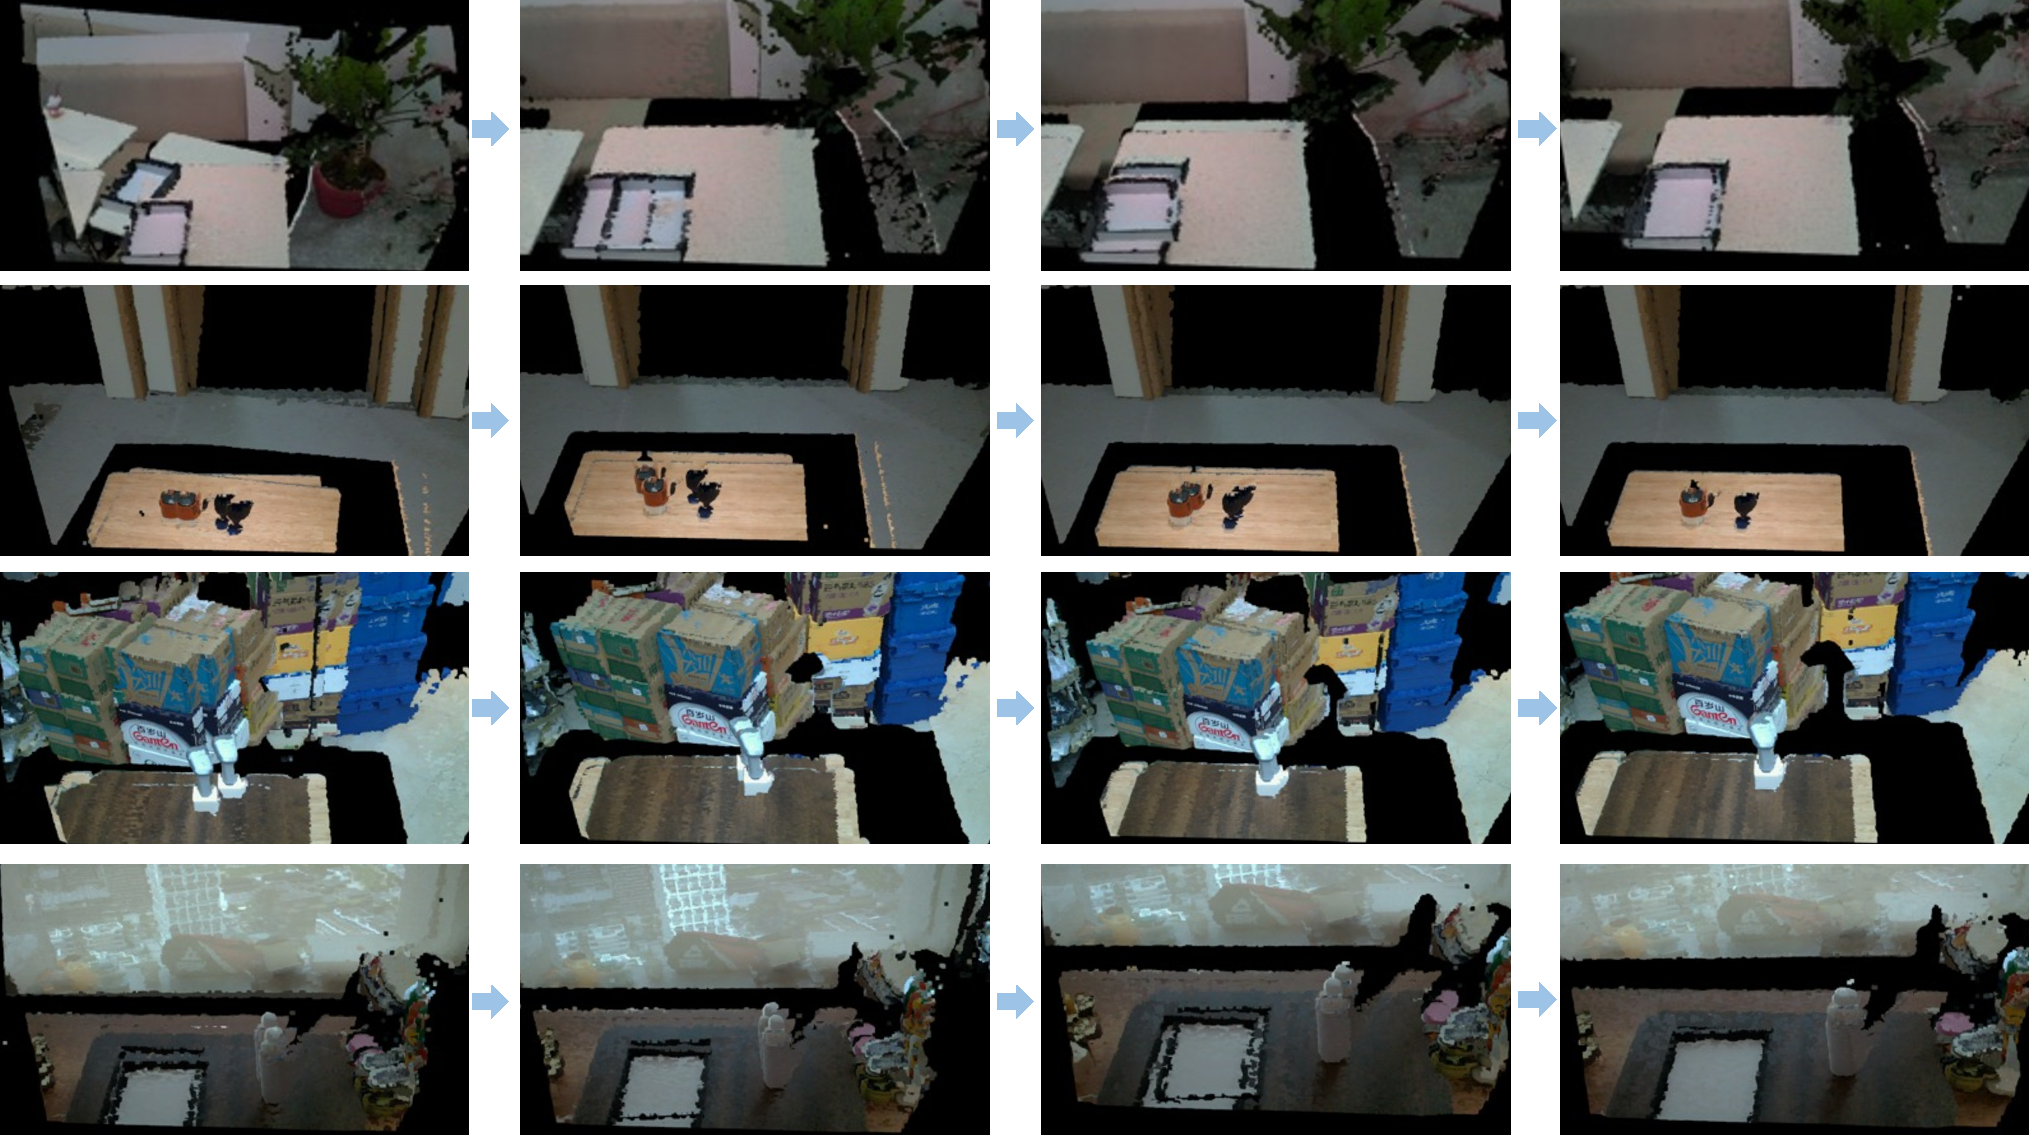
\includegraphics[width=1.0\linewidth]{figures/closed-loop-PnP_pic.pdf}
  \caption{\textbf{Closed-loop PnP visualization.} Across diverse scenarios, the closed-loop PnP algorithm iteratively refines the robot’s pose and ultimately aligns it with the desired target pose with high precision.}
  \label{fig:closed-loop}
\end{figure*}




\subsection{Qualitative Analysis of Closed-loop PnP}

Figure~\ref{fig:closed-loop} illustrates that across various scenarios, the closed-loop PnP localization with iterative refinements progressively aligns the captured point clouds with the target positions, underscoring the localization precision achieved by \ourshort.


\subsection{DAgger Training}
\label{sec:dagger_train}
Regarding DAgger training, we compare our implementation of DAgger with both pure expert training~(i.e., Behavior Cloning) and pure student training. Figure~\ref{fig:dagger_curves} reports each method’s performance on two representative tasks. \textit{Clean Table} is a long-horizon task in which the robot must first place two objects into a box and then move the box to the center of the table. As shown in Figure~\ref{fig:dagger_curves}, pure imitation learning struggles to cover long-horizon and out-of-distribution states. In \textit{Clean Plate}, where the human motion is extracted from raw videos, the expert policy’s actions contain non-negligible noise; consequently, during early interactive training, action errors can be amplified by querying this noisy expert, leading to poor sample efficiency. In contrast, HERMES warms up the policy with expert data and then gradually reduces reliance on the expert action distribution, achieving high sample efficiency without sacrificing asymptotic performance in both tasks.

\begin{figure}[h]
  \centering
  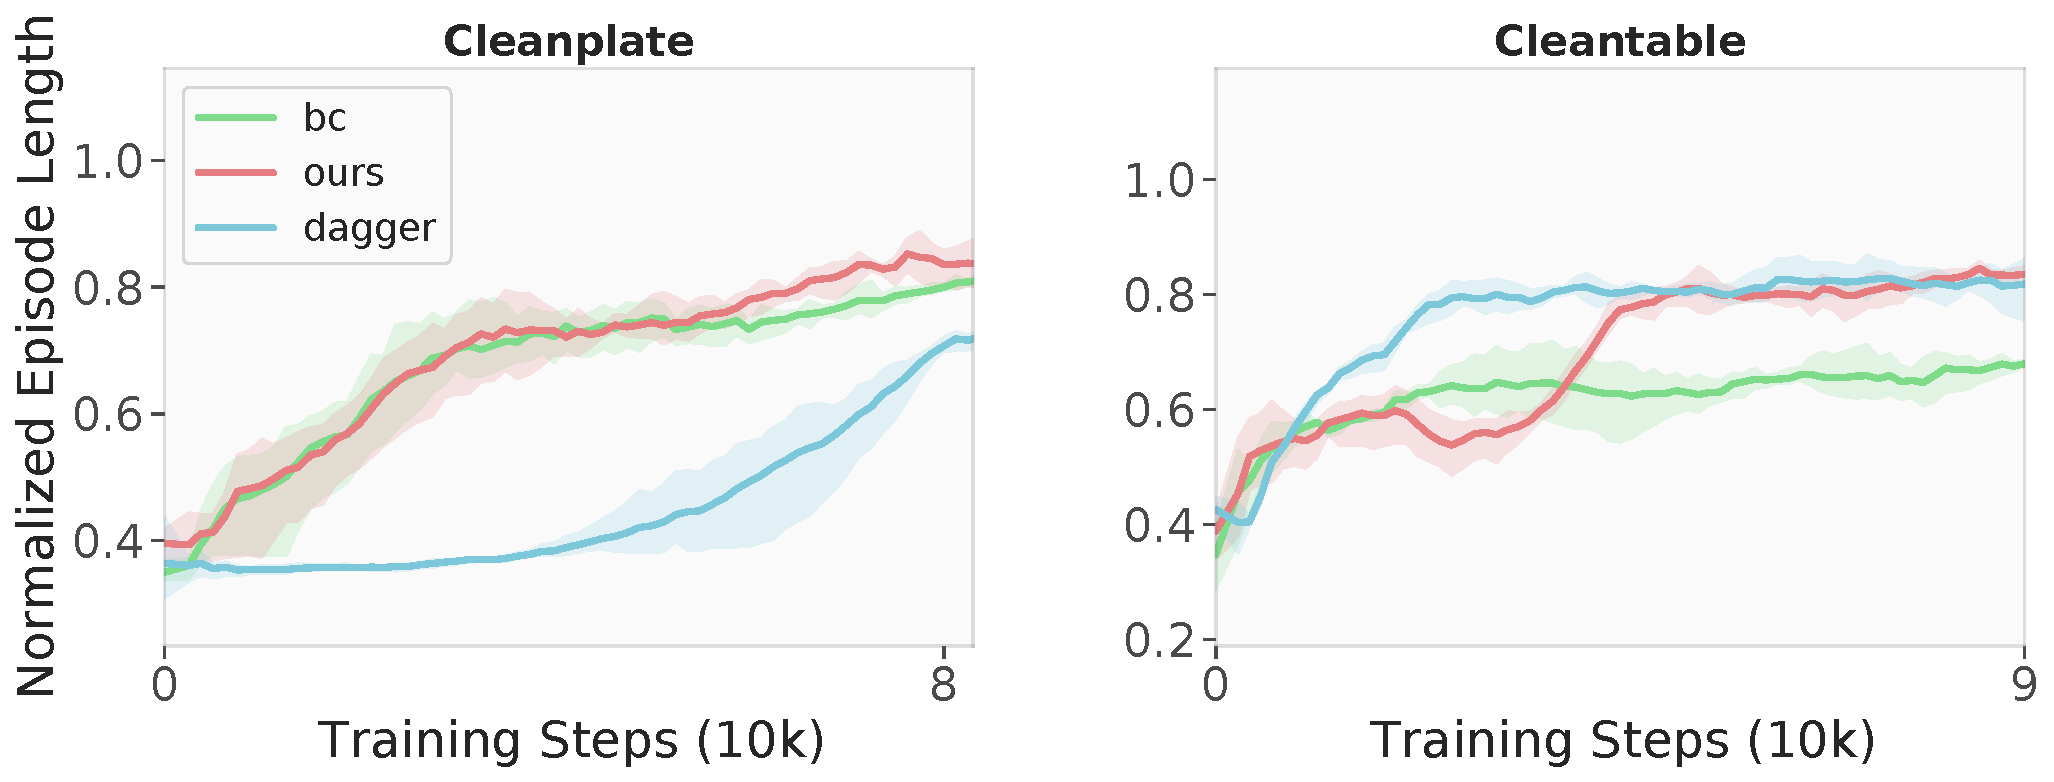
\includegraphics[width=1.0\linewidth]{figures/dagger_curves_pic.pdf}
  \caption{ \textbf{DAgger training efficiency.} \ourshort attains high sample efficiency and asymptotic performance across different types of tasks.}
  \label{fig:dagger_curves}
\end{figure}



\subsection{Hybrid Control for Real-world Evaluation}
\label{sec:hybrid}
\begin{figure}[t]
  \centering
  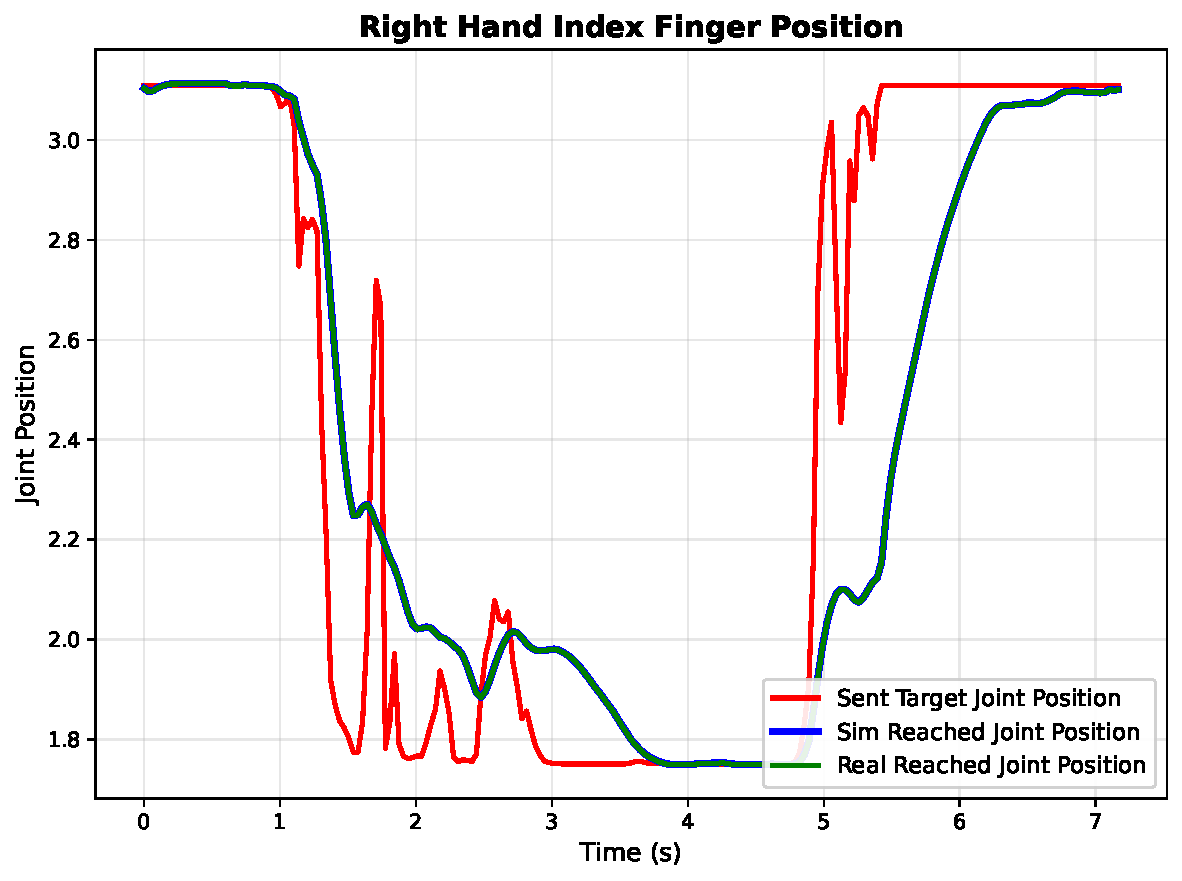
\includegraphics[width=0.9\linewidth]{figures/hybrid-control_pic.pdf}
  \caption{ \textbf{The comparison of sent target joint position and the actual reached joint position in both simulation and real-world.} The red, blue, and green curves exhibit similar overall trends. Compared with the blue and green curves, the red curve shows a deviation in joint position at the same time step, while the blue and green traces overlaps throughout. This discrepancy points to the gap between the simulated and real-world dynamics, and adopting the hybrid control keeping the dynamics consistency between the simulation and the real robot.}
  \label{fig:hybrid-control}
\end{figure}
It is worth noting that, in our hybrid sim2real control framework, the simulation environment does not contain any object models. We rely on the simulated robot to carry out all kinematic and dynamic computations and to maintain alignment with the real system. Furthermore, to showcase the benefits of our hybrid sim2real control strategy, we visualize the temporal trajectory of the right-hand index-finger joint angle during policy execution. Figure~\ref{fig:hybrid-control} shows a pronounced, nonlinear discrepancy between the joint target position inferred by the policy and the actual reached joint position. Such a sizable mismatch is difficult for the policy to compensate for. In contrast, the hybrid sim2real control strategy forces the simulated and real robots to share an identical dynamics model. As demonstrated in Figure~\ref{fig:hybrid-control}, the blue and green traces remain consistently overlapped across the entire horizon, indicating that hybrid control substantially reduces the sim2real gap.


\subsection{The Sequential Adjustment Strategy of Closed-loop PnP}

During the closed-loop PnP stage, the system takes a goal RGBD image $I_g$ and a current robot-captured RGBD image $I_c$ as inputs. At each timestep $t$, the robot updates $I_c$ with its current view. The $\text{PnP}$ algorithm which is made up of RANSAC PnP \cite{zuliani2009ransac} and refine PnP \cite{madsen2004methods,eade2013gauss,bradski2000opencv} computes the relative rotation $\mathbf{R} \in \mathbb{R}^{3\times 3}$ and translation $\mathbf{t} \in \mathbb{R}^3$ between the current and goal poses. The pose errors in x direction, y direction and yaw orientation are derived as $e_{\text{x}}$, $e_{\text{y}}$, $e_{\text{yaw}}$ from the relative rotation and translation. These errors drive the PID controller \cite{willis1999proportional} to output $v_{\text{x}}$, $v_{\text{y}}$, $v_{\text{yaw}}$, which move the robot base to reduce the errors. The adjustment loop terminates when all errors satisfy $|e_j| < \varepsilon_j$ for $j \in {\text{x, y, yaw}}$.

\begin{algorithm}
\caption{Closed-loop PnP Adjustment}\label{alg:PnP}
\begin{algorithmic}
\Require Goal RGBD image $I_g$, thresholds $\varepsilon_{\text{x}}$, $\varepsilon_{\text{y}}$, $\varepsilon_{\text{yaw}}$
\Ensure Adjusted robot pose
\State Initialize PID controllers
\While{$\max\left( \frac{|e_{\text{x}}|}{\varepsilon_{\text{x}}}, \frac{|e_{\text{y}}|}{\varepsilon_{\text{y}}}, \frac{|e_{\text{yaw}}|}{\varepsilon_{\text{yaw}}} \right) > 1$}
    \State Capture current RGBD image $I_c$
    \State $\mathbf{R}, \mathbf{t} \gets \text{PnP}(I_g, I_c)$ \Comment{Using RANSAC + Refine PnP}
    \For{$j \in \{\text{x, y, yaw}\}$}
        \State $e_j  \gets\text{ExtractPoseErrors}(\mathbf{R,T})$
        \State $v_j \gets \text{PIDController}(e_j)$
    \EndFor
    \State Send velocity command $(v_{\text{x}}, v_{\text{y}}, v_{\text{yaw}})$ to robot
\EndWhile
\end{algorithmic}
\end{algorithm}




\begin{figure*}[t]
  \centering
  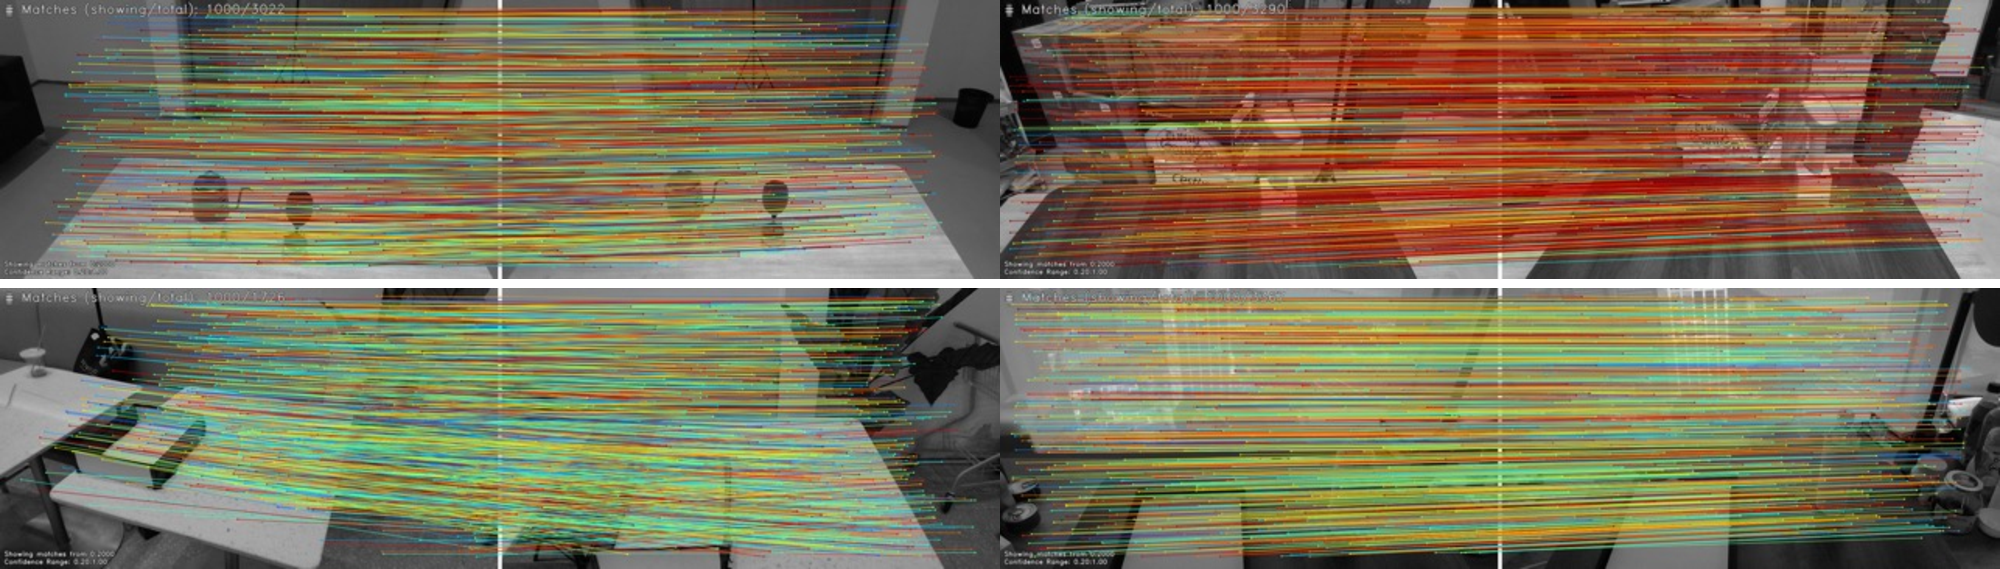
\includegraphics[width=1.0\linewidth]{figures/feature-matcher_pic.pdf}
  \caption{ \textbf{Feature matcher visualization of Efficient LoFTR.} Efficient LoFTR is capable of establishing correspondences between the target RGB image and the current RGB frame at a high frequency.}
  \label{fig:feature}
\end{figure*}
\subsection{Feature Matcher Visualization}

Efficient LoFTR~\cite{wang2024efficient} consistently extracts dense feature correspondences at high frequency across various environments. This capability provides the rich feature correspondence required for the subsequent PnP pose estimation. The visualizations are shown in Figure~\ref{fig:feature}. 


\subsection{Comparison with the depth image from Depth Anything }
\begin{figure}[t]
  \centering
  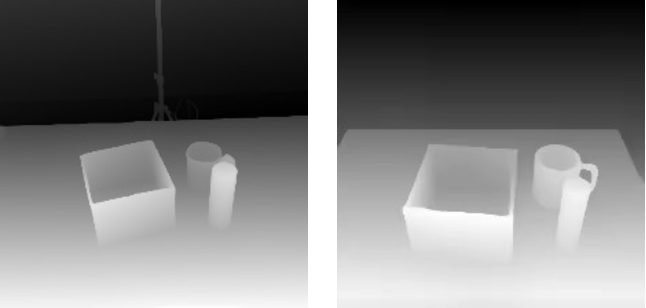
\includegraphics[width=0.9\linewidth]{figures/dpt-compare_pic.pdf}
  \caption{ \textbf{Comparison of Depth-anything generated images between simulation and real-world.} Depth-Anything can produce depth images that are semantically aligned between simulation and real-world.}
  \label{fig:dpt-compare}
\end{figure}
\begin{figure}[h]
  \centering
  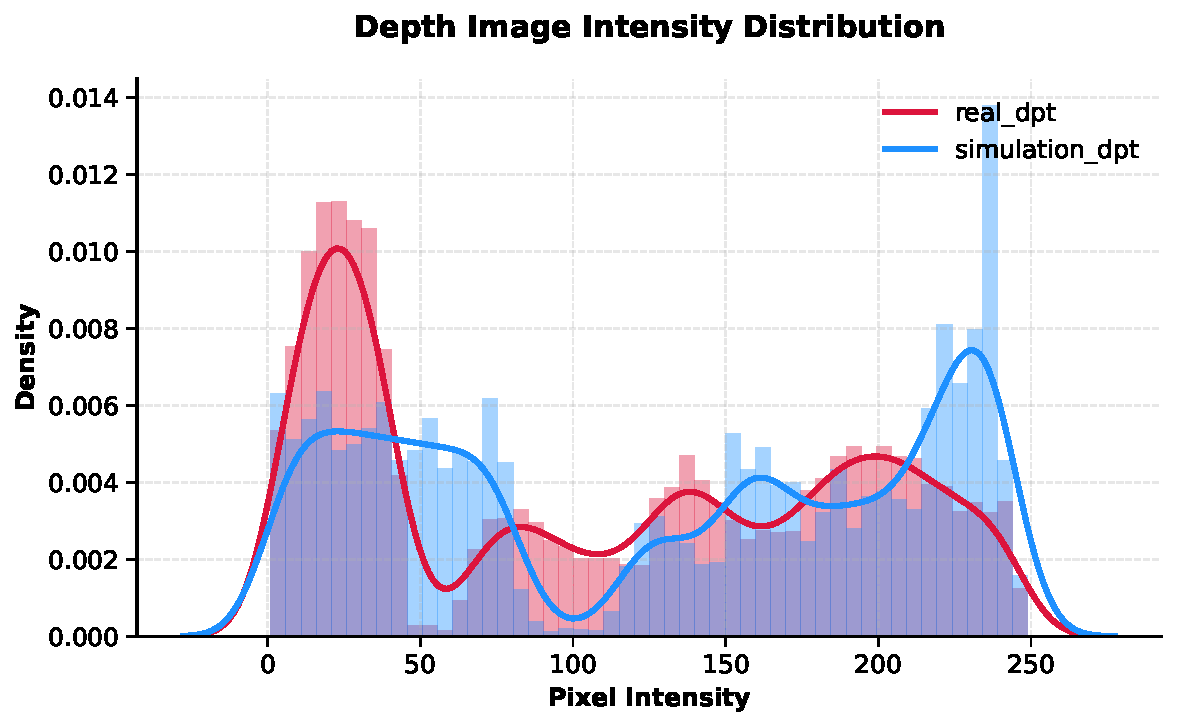
\includegraphics[width=1.0\linewidth]{figures/dpt-dist_pic.pdf}
  \caption{\textbf{Depth intensity distribution of Depth-anything generated images. }The red curve shows the depth-value distribution extracted from real-world RGB images, whereas the blue curve corresponds to that obtained from simulated images. Despite their semantic alignment, the depth maps estimated by Depth-Anything reveal a pronounced quantitative gap between the simulated and real-world domains.}
  \label{fig:dpt_dist}
\end{figure}
Depth-Anything~\cite{yang2024depth,yang2024depth2}, a widely adopted foundation model for depth estimation, demonstrates remarkable robustness and fine-grained detail perception, even under diverse and unstructured real-world conditions. Building on these capabilities, we also leverage Depth-Anything to bridge the perceptual gap between simulation and the real world. Consistent with \ourshort, we also apply the \textit{mixup} augmentation strategy with the disparity map to enhance the robustness. We first utilize the NYU Depth Dataset~\cite{silberman2012indoor} and transform the depth maps $D$ into disparity maps $\hat{I}$ to better align with the  distribution of DA generated images:
\begin{equation}
    \hat{I}(x, y) = \frac{1}{D(x, y)},
\end{equation}
where $(x, y)$ is the pixel position.

We then blend the DA input $\boldsymbol{o}_{DA}$ with a certain disparity map $\boldsymbol{o}_{disparity}$: ${\boldsymbol{\hat{o}}} = \alpha*\boldsymbol{o}_{DA} + (1 - \alpha)*\boldsymbol{o}_{disparity}$, where $\alpha$ is the coefficient. ${\boldsymbol{\hat{o}}}$ is then used as the final visual input to the network.

We compare our  depth-augmentation scheme with the depth maps synthesized by Depth-anything-v2. As reported in Table~\ref{table: compare_da}, \ourshort achieves better performance and success rates. Although Figure~\ref{fig:dpt-compare} shows that the synthetic depth maps can achieve semantic coherence between simulation and real-world depth estimation, Figure~\ref{fig:dpt_dist} reveals a distributional discrepancy in the underlying pixel-wise depth estimates across the two domains. This numerical gap ultimately suppresses overall success rates, making the method less effective than our direct preprocessing of raw depth images.


\begin{table}[h]
\centering
\caption{Comparison of \ourshort and Depth-Anything}
\label{table: compare_da}
\resizebox{0.4\textwidth}{!}{
\begin{tabular}{c|cc}
\toprule

\begin{tabular}[c]{@{}c@{}} \multicolumn{1}{c}{\multirow{1}{*}{Tasks $\backslash$ Method}} \end{tabular}   & \multicolumn{1}{c}{\ourshort} & \multicolumn{1}{c}{Depth-Anything} \\

\midrule

Bottle Handover & \best{66.7} & $40.0$  \\

Scan Bottle &	\best{73.3} & $33.3$  \\

\bottomrule
\end{tabular}
}
\end{table}




